\subsection{Transformed\-Image  Class Reference}
\label{class_transformedimage}\index{TransformedImage@{Transformed\-Image}}
class that operates the transformation of a {\bf Reduced\-Image} {\rm (p.\,\pageref{class_reducedimage})} (image(s) + list). 


{\tt \#include $<$transformedimage.h$>$}

Inheritance diagram for Transformed\-Image::\begin{figure}[H]
\begin{center}
\leavevmode
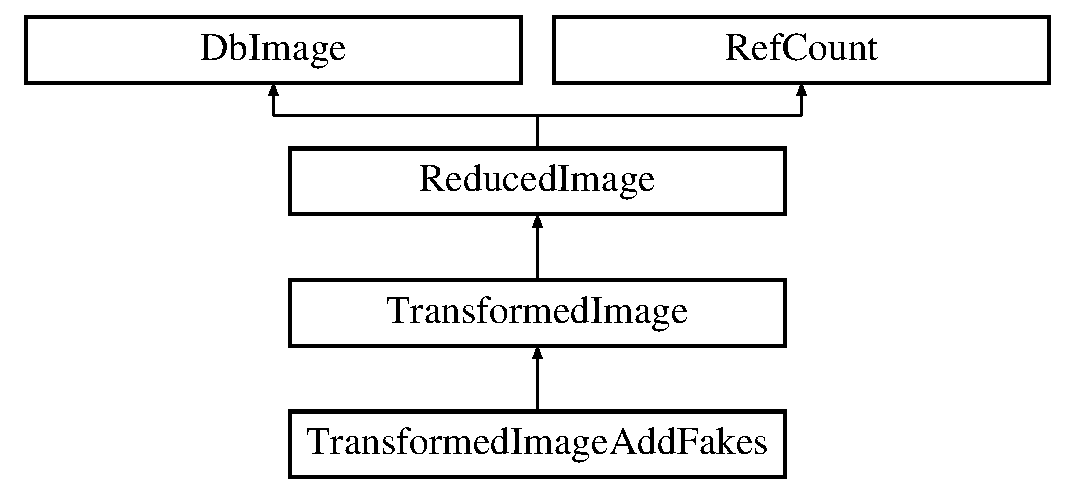
\includegraphics[height=4cm]{class_transformedimage}
\end{center}
\end{figure}
\subsubsection*{Public Methods}
\begin{CompactItemize}
\item 
{\bf Transformed\-Image} (const string \&Name, const {\bf Reduced\-Image} \&Source, const Image\-Transfo $\ast$Transfo)
\begin{CompactList}\small\item\em to create a new Transformed\-Image, or locate an existing one.\item\end{CompactList}\item 
\index{TransformedImage@{TransformedImage}!TransformedImage@{Transformed\-Image}}\index{TransformedImage@{TransformedImage}!TransformedImage@{Transformed\-Image}}
{\bf Transformed\-Image} (const string \&Name)\label{class_transformedimage_a1}

\begin{CompactList}\small\item\em assumes that the Transformed\-Image already exists.\item\end{CompactList}\item 
\index{TransformedImage@{TransformedImage}!TransformedImage@{Transformed\-Image}}\index{TransformedImage@{TransformedImage}!TransformedImage@{Transformed\-Image}}
{\bf Transformed\-Image} ()\label{class_transformedimage_a2}

\item 
\index{SourceName@{SourceName}!TransformedImage@{Transformed\-Image}}\index{TransformedImage@{TransformedImage}!SourceName@{Source\-Name}}
string {\bf Source\-Name} () const\label{class_transformedimage_a3}

\begin{CompactList}\small\item\em Original (untransformed) image name.\item\end{CompactList}\item 
\index{Source@{Source}!TransformedImage@{Transformed\-Image}}\index{TransformedImage@{TransformedImage}!Source@{Source}}
{\bf Reduced\-Image}$\ast$ {\bf Source} () const\label{class_transformedimage_a4}

\begin{CompactList}\small\item\em Original (untransformed) image.\item\end{CompactList}\item 
\index{GeometricReference@{GeometricReference}!TransformedImage@{Transformed\-Image}}\index{TransformedImage@{TransformedImage}!GeometricReference@{Geometric\-Reference}}
{\bf Reduced\-Image}$\ast$ {\bf Geometric\-Reference} ()\label{class_transformedimage_a5}

\begin{CompactList}\small\item\em Geometric reference (only applicable if Image\-Transfo is {\bf Image\-Gtransfo} {\rm (p.\,\pageref{class_imagegtransfo})}).\item\end{CompactList}\item 
\index{Transfo@{Transfo}!TransformedImage@{Transformed\-Image}}\index{TransformedImage@{TransformedImage}!Transfo@{Transfo}}
const Image\-Transfo$\ast$ {\bf Transfo} () const\label{class_transformedimage_a6}

\begin{CompactList}\small\item\em involved transformation.\item\end{CompactList}\item 
\index{FromRef@{FromRef}!TransformedImage@{Transformed\-Image}}\index{TransformedImage@{TransformedImage}!FromRef@{From\-Ref}}
const {\bf Gtransfo}$\ast$ {\bf From\-Ref} () const\label{class_transformedimage_a7}

\begin{CompactList}\small\item\em {\bf Gtransfo} {\rm (p.\,\pageref{class_gtransfo})} from reference to transformed image. Assumes that Image\-Transfo is an {\bf Image\-Gtransfo} {\rm (p.\,\pageref{class_imagegtransfo})}.\item\end{CompactList}\item 
\index{dump@{dump}!TransformedImage@{Transformed\-Image}}\index{TransformedImage@{TransformedImage}!dump@{dump}}
virtual void {\bf dump} (ostream \&s=cout) const\label{class_transformedimage_a8}

\begin{CompactList}\small\item\em dumps basic info.\item\end{CompactList}\item 
\index{MakeFits@{MakeFits}!TransformedImage@{Transformed\-Image}}\index{TransformedImage@{TransformedImage}!MakeFits@{Make\-Fits}}
virtual bool {\bf Make\-Fits} ()\label{class_transformedimage_a9}

\begin{CompactList}\small\item\em produce fits image.\item\end{CompactList}\item 
\index{MakeCatalog@{MakeCatalog}!TransformedImage@{Transformed\-Image}}\index{TransformedImage@{TransformedImage}!MakeCatalog@{Make\-Catalog}}
virtual bool {\bf Make\-Catalog} ()\label{class_transformedimage_a10}

\begin{CompactList}\small\item\em Produce the Saturated stars pixels mask, subtract the image background, detect with the SExtractor computed sigma. search the cosmics, and update catalog and weight for cosmics. No free coffee.\item\end{CompactList}\item 
\index{MakeDead@{MakeDead}!TransformedImage@{Transformed\-Image}}\index{TransformedImage@{TransformedImage}!MakeDead@{Make\-Dead}}
virtual bool {\bf Make\-Dead} ()\label{class_transformedimage_a11}

\begin{CompactList}\small\item\em produce dead image.\item\end{CompactList}\item 
\index{MakeSatur@{MakeSatur}!TransformedImage@{Transformed\-Image}}\index{TransformedImage@{TransformedImage}!MakeSatur@{Make\-Satur}}
virtual bool {\bf Make\-Satur} ()\label{class_transformedimage_a12}

\begin{CompactList}\small\item\em produce satur image.\item\end{CompactList}\item 
\index{MakeCosmic@{MakeCosmic}!TransformedImage@{Transformed\-Image}}\index{TransformedImage@{TransformedImage}!MakeCosmic@{Make\-Cosmic}}
virtual bool {\bf Make\-Cosmic} ()\label{class_transformedimage_a13}

\begin{CompactList}\small\item\em produce cosmic image.\item\end{CompactList}\item 
\index{MakeSatellite@{MakeSatellite}!TransformedImage@{Transformed\-Image}}\index{TransformedImage@{TransformedImage}!MakeSatellite@{Make\-Satellite}}
virtual bool {\bf Make\-Satellite} ()\label{class_transformedimage_a14}

\begin{CompactList}\small\item\em produce satellite image.\item\end{CompactList}\item 
\index{MakeWeight@{MakeWeight}!TransformedImage@{Transformed\-Image}}\index{TransformedImage@{TransformedImage}!MakeWeight@{Make\-Weight}}
virtual bool {\bf Make\-Weight} ()\label{class_transformedimage_a15}

\item 
\index{Create@{Create}!TransformedImage@{Transformed\-Image}}\index{TransformedImage@{TransformedImage}!Create@{Create}}
bool {\bf Create} (const string \&Where)\label{class_transformedimage_a16}

\begin{CompactList}\small\item\em To create the directories where the fits images, catalogues will be put: ex: $\sim$/Fake\-Db/test: {\bf Db\-Image} {\rm (p.\,\pageref{class_dbimage})} dbim(\char`\"{}test\char`\"{}); dbim.Create(\char`\"{}$\sim$/Fake\-Db/\char`\"{});.\item\end{CompactList}\item 
\index{Clone@{Clone}!TransformedImage@{Transformed\-Image}}\index{TransformedImage@{TransformedImage}!Clone@{Clone}}
{\bf Reduced\-Image}$\ast$ {\bf Clone} () const\label{class_transformedimage_a17}

\item 
\index{TransformedImage@{TransformedImage}!TransformedImage@{Transformed\-Image}}\index{TransformedImage@{TransformedImage}!TransformedImage@{Transformed\-Image}}
{\bf Transformed\-Image} (const Transformed\-Image \&Original)\label{class_transformedimage_a18}

\item 
\index{~TransformedImage@{$\sim$TransformedImage}!TransformedImage@{Transformed\-Image}}\index{TransformedImage@{TransformedImage}!~TransformedImage@{$\sim$Transformed\-Image}}
{\bf $\sim$Transformed\-Image} ()\label{class_transformedimage_a19}

\end{CompactItemize}


\subsubsection{Detailed Description}
class that operates the transformation of a {\bf Reduced\-Image} {\rm (p.\,\pageref{class_reducedimage})} (image(s) + list).

As for other descendants of {\bf Reduced\-Image} {\rm (p.\,\pageref{class_reducedimage})}, the actual computations occur when you request the name of a data file (e.g. {\bf Fits\-Name}() {\rm (p.\,\pageref{class_reducedimage_a14})}). To geometrically align a set of images on the same reference, use Images\-Align(). If you want to sum them, uses Images\-Align\-And\-Sum() 



\subsubsection{Constructor \& Destructor Documentation}
\index{TransformedImage@{Transformed\-Image}!TransformedImage@{TransformedImage}}
\index{TransformedImage@{TransformedImage}!TransformedImage@{Transformed\-Image}}
\paragraph{\setlength{\rightskip}{0pt plus 5cm}Transformed\-Image::Transformed\-Image (const string \& {\em Name}, const {\bf Reduced\-Image} \& {\em Source}, const Image\-Transfo $\ast$ {\em Transfo})}\hfill\label{class_transformedimage_a0}


to create a new Transformed\-Image, or locate an existing one.

If you want to align A on B, the typical constructor call will be: Transformed\-Image(New\-Name, A, \&Image\-Gtransfo(B,A)); To align a set of images on the same reference, use Images\-Align(). 

The documentation for this class was generated from the following file:\begin{CompactItemize}
\item 
{\bf transformedimage.h}\end{CompactItemize}
